% =============================================================================
%  main.tex — корневой файл статьи (arXiv preprint)
%  Сборка:  latexmk -pdf main.tex   или   make
%  Пакет для arXiv:  make arxiv   (создаёт arxiv_submission.tar.gz)
% =============================================================================
\documentclass[10pt,a4paper,twocolumn]{article}
% Для одноколоночного варианта (удобно для черновика) замените на:
% \documentclass[11pt,a4paper]{article}

% =============================================================================
%  preamble.tex — подключение пакетов
%  Все пакеты входят в TeX Live и доступны на сервере arXiv.
% =============================================================================

% --- Кодировка, шрифты, язык ------------------------------------------------
\usepackage[utf8]{inputenc}
\usepackage[T1]{fontenc}
\usepackage{lmodern}
\usepackage{microtype}
\usepackage[english]{babel}
% Если нужны русские вставки (например, в комментариях к рисункам):
% \usepackage[T2A,T1]{fontenc}
% \usepackage[russian,english]{babel}

% --- Геометрия страницы ----------------------------------------------------
\usepackage[margin=2cm,columnsep=0.8cm]{geometry}

% --- Математика ------------------------------------------------------------
\usepackage{amsmath,amssymb,amsfonts,amsthm,mathtools}
\usepackage{bm}

% --- Графика и рисунки -----------------------------------------------------
\usepackage{graphicx}
\graphicspath{{figures/}}
\usepackage{xcolor}
\usepackage{tikz}
\usetikzlibrary{arrows.meta,positioning,shapes.geometric,fit,calc,backgrounds}
\usepackage[caption=false,font=footnotesize]{subfig}
\usepackage{float}

% --- Таблицы ---------------------------------------------------------------
\usepackage{booktabs}
\usepackage{multirow}
\usepackage{tabularx}
\usepackage{makecell}
\usepackage{threeparttable}

% --- Единицы измерения (мВт, МГц, мм^2 ...) ---------------------------------
\usepackage{siunitx}
\sisetup{detect-all, range-phrase = --, per-mode = symbol}

% --- Алгоритмы -------------------------------------------------------------
\usepackage{algorithm}
\usepackage{algpseudocode}

% --- Листинги (Verilog/SystemVerilog, C++) -----------------------------------
\usepackage{listings}
\lstset{
  basicstyle=\ttfamily\footnotesize,
  keywordstyle=\color{blue!70!black}\bfseries,
  commentstyle=\color{green!45!black},
  stringstyle=\color{red!60!black},
  numbers=left, numberstyle=\tiny, frame=single,
  breaklines=true, columns=fullflexible, captionpos=b,
}

% --- Библиография (natbib + BibTeX: arXiv принимает готовый .bbl) -------------
\usepackage[numbers,sort&compress]{natbib}

% --- Прочее ------------------------------------------------------------------
\usepackage{xspace}
\usepackage{enumitem}
\setlist{nosep}
\usepackage{url}
\usepackage{todonotes}   % \todo{...}; для финальной версии: [disable]

% --- Гиперссылки (подключать последними) -----------------------------------
\usepackage[hidelinks,breaklinks]{hyperref}
\usepackage[nameinlink,capitalise,noabbrev]{cleveref}

% --- Теоремы / определения -------------------------------------------------
\newtheorem{definition}{Definition}
\newtheorem{proposition}{Proposition}

% =============================================================================
%  macros.tex — пользовательские команды
% =============================================================================

% --- Пометки для работы над текстом ----------------------------------------
% Чтобы скрыть все пометки в финальной версии: \renewcommand{\TODO}[1]{}
\newcommand{\TODO}[1]{\textcolor{red}{\textbf{[TODO: #1]}}}
\newcommand{\NOTE}[1]{\textcolor{blue}{\textit{[Note: #1]}}}
\newcommand{\CITE}{\textcolor{orange}{\textbf{[cite]}}}
\newcommand{\NUM}{\textcolor{red}{\textbf{XX}}}   % заглушка для чисел

% --- Название системы (поменять в одном месте) ------------------------------
\newcommand{\sysname}{\textsc{DH-SLAM-1}\xspace}

% --- Сокращения ------------------------------------------------------------
\newcommand{\eg}{e.g.,\xspace}
\newcommand{\ie}{i.e.,\xspace}
\newcommand{\etal}{\textit{et al.}\xspace}
\newcommand{\wrt}{w.r.t.\xspace}

% --- Математические обозначения (SLAM) --------------------------------------
\newcommand{\R}{\mathbb{R}}
\newcommand{\SE}[1]{\mathrm{SE}(#1)}
\newcommand{\SO}[1]{\mathrm{SO}(#1)}
\newcommand{\pose}{\mathbf{T}}            % поза камеры
\newcommand{\rot}{\mathbf{R}}             % вращение
\newcommand{\trans}{\mathbf{t}}           % перенос
\newcommand{\landmark}{\mathbf{p}}        % 3D-точка карты
\newcommand{\meas}{\mathbf{z}}            % измерение
\newcommand{\state}{\mathbf{x}}           % вектор состояния
\newcommand{\jac}{\mathbf{J}}             % якобиан
\newcommand{\hess}{\mathbf{H}}            % (приближённый) гессиан
\newcommand{\infomat}{\boldsymbol{\Omega}}% информационная матрица
\newcommand{\norm}[1]{\left\lVert#1\right\rVert}
\DeclareMathOperator*{\argmin}{arg\,min}

% --- Аппаратные метрики -----------------------------------------------------
\newcommand{\fps}{\,FPS}
\newcommand{\mJpf}{\,\si{\milli\joule}/frame}


% ----------------------------------------------------------------------------
%  Метаданные
% ----------------------------------------------------------------------------
\title{%
  \An Energy-Efficient ASIC Accelerator\\
  for Real-Time Visual-Inertial SLAM%
}

\author{%
  Magamed Abdulvadudov\thanks{Corresponding author: \texttt{sbryukov@gmail.com}}\\
  \small \TODO{Affiliation, City, Country}
  \and
  Sergey Bryukov\\
  \small {SkolTech, Moscow, Russia}
}

\date{\today}

\hypersetup{
  pdftitle    = {An Energy-Efficient ASIC Accelerator for Real-Time Visual-Inertial SLAM},
  pdfauthor   = {Sergey Bryukov},
  pdfkeywords = {SLAM, ASIC, hardware accelerator, visual odometry, low power, robotics},
}

% ============================================================================
\begin{document}

\twocolumn[
  \begin{@twocolumnfalse}
    \maketitle
    % =============================================================================
%  Abstract (arXiv: <= 1920 символов в форме подачи; текст в PDF может совпадать)
%  Структура: контекст -> проблема -> что сделано -> ключевые числа -> вывод
% =============================================================================
\begin{abstract}
Simultaneous Localization and Mapping (SLAM) is a core capability of
autonomous robots, drones, and AR/VR headsets, yet state-of-the-art
algorithms remain too power-hungry for milliwatt-class edge platforms. The bottleneck of modern Edge AI SoC is memory bus and DMA are highly loads while data transferring before computation, also computation blocs such as NPU/TPU/GPU have general architecture and not optimized for SLAM. Specifically to SLAM and other sensor data processing, moving data from camera to CPU, feature extraction and then passing to computation block dominate latency and energy on SoC. In this paper we present \sysname, a \TODO{process node, e.g., 28-nm CMOS}
ASIC accelerator for \TODO{visual / visual-inertial} SLAM that
\TODO{key idea 1, e.g., a streaming feature front-end} and
\TODO{key idea 2, e.g., a sparse Schur-complement back-end with on-chip
marginalization}.
The chip occupies \NUM~\si{\milli\metre\squared}, runs at \NUM~\si{\mega\hertz},
and processes \NUM\fps\ VGA input while consuming \NUM~\si{\milli\watt}
--- \NUM$\times$ more energy-efficient than \TODO{baseline platform}
with \TODO{no / $<$X\%} accuracy degradation on the EuRoC and TUM RGB-D
benchmarks.
\TODO{One-sentence take-away / availability of RTL or dataset.}
\end{abstract}

\noindent\textbf{Keywords:} SLAM, ASIC, hardware accelerator, visual odometry,
bundle adjustment, energy efficiency, edge robotics.

    \vspace{1em}
  \end{@twocolumnfalse}
]
% Для одноколоночного режима удалите блок \twocolumn[...] выше и раскомментируйте:
% \maketitle
% % =============================================================================
%  Abstract (arXiv: <= 1920 символов в форме подачи; текст в PDF может совпадать)
%  Структура: контекст -> проблема -> что сделано -> ключевые числа -> вывод
% =============================================================================
\begin{abstract}
Simultaneous Localization and Mapping (SLAM) is a core capability of
autonomous robots, drones, and AR/VR headsets, yet state-of-the-art
algorithms remain too power-hungry for milliwatt-class edge platforms. The bottleneck of modern Edge AI SoC is memory bus and DMA are highly loads while data transferring before computation, also computation blocs such as NPU/TPU/GPU have general architecture and not optimized for SLAM. Specifically to SLAM and other sensor data processing, moving data from camera to CPU, feature extraction and then passing to computation block dominate latency and energy on SoC. In this paper we present \sysname, a \TODO{process node, e.g., 28-nm CMOS}
ASIC accelerator for \TODO{visual / visual-inertial} SLAM that
\TODO{key idea 1, e.g., a streaming feature front-end} and
\TODO{key idea 2, e.g., a sparse Schur-complement back-end with on-chip
marginalization}.
The chip occupies \NUM~\si{\milli\metre\squared}, runs at \NUM~\si{\mega\hertz},
and processes \NUM\fps\ VGA input while consuming \NUM~\si{\milli\watt}
--- \NUM$\times$ more energy-efficient than \TODO{baseline platform}
with \TODO{no / $<$X\%} accuracy degradation on the EuRoC and TUM RGB-D
benchmarks.
\TODO{One-sentence take-away / availability of RTL or dataset.}
\end{abstract}

\noindent\textbf{Keywords:} SLAM, ASIC, hardware accelerator, visual odometry,
bundle adjustment, energy efficiency, edge robotics.


% =============================================================================
\section{Introduction}
\label{sec:intro}
% =============================================================================
% План: (1) мотивация -> (2) почему существующие платформы не подходят ->
% (3) наш подход -> (4) вклад (bullet list) -> (5) структура статьи

% --- (1) Мотивация ---------------------------------------------------------
Accurate, low-latency ego-motion estimation and mapping is a prerequisite for
autonomous navigation of micro aerial vehicles, mobile robots, and
head-mounted AR/VR devices~\cite{cadena2016past}.
Modern feature-based and direct SLAM systems such as
ORB-SLAM3~\cite{campos2021orbslam3} and VINS-Mono~\cite{qin2018vins}
achieve centimeter-level accuracy, but \TODO{quantify: power / latency on
embedded CPU (e.g., \NUM~W on Jetson-class SoC)}.

% --- (2) Проблема ------------------------------------------------------------
\TODO{Explain the gap: power budget of target platforms (e.g., nano-drones
$<$\NUM~mW for compute), memory bandwidth limits, irregular sparse workloads
in the back-end that map poorly to GPUs.}
Prior accelerators~\cite{suleiman2019navion,li2019cnn_slam_asic}
\TODO{what they did and what they miss}.

% --- (3) Подход --------------------------------------------------------------
To address these challenges, we propose \sysname, \TODO{one-paragraph
description of the architecture and the central insight}.

% --- (4) Вклад -------------------------------------------------------------
The main contributions of this work are:
\begin{itemize}
  \item \TODO{Contribution 1: algorithm--hardware co-design, e.g.,
        hardware-friendly reformulation of \ldots};
  \item \TODO{Contribution 2: micro-architecture, e.g., streaming front-end
        with \NUM~KB line buffers instead of full-frame storage};
  \item \TODO{Contribution 3: silicon implementation and measurement in
        \NUM-nm CMOS};
  \item \TODO{Contribution 4: comprehensive evaluation against CPU, GPU,
        FPGA and ASIC baselines on public datasets}.
\end{itemize}

% --- (5) Структура -----------------------------------------------------------
The remainder of the paper is organized as follows.
\Cref{sec:related} reviews related work.
\Cref{sec:background} summarizes the SLAM pipeline and profiles its
computational bottlenecks.
\Cref{sec:architecture} presents the proposed architecture, and
\cref{sec:implementation} describes its physical implementation.
\Cref{sec:evaluation} reports experimental results,
\cref{sec:discussion} discusses limitations, and
\cref{sec:conclusion} concludes the paper.

% =============================================================================
\section{Related Work}
\label{sec:related}
% =============================================================================
% Группировать работы по темам; в конце каждого абзаца — чем наша работа отличается.

\subsection{SLAM Algorithms}
Feature-based methods~\cite{mur2015orbslam,campos2021orbslam3},
direct methods~\cite{engel2018dso}, and tightly coupled
visual-inertial estimators~\cite{qin2018vins,forster2017preintegration}
\TODO{short overview; which class our accelerator targets and why}.

\subsection{SLAM on Embedded CPUs, GPUs and FPGAs}
\TODO{Embedded software implementations, GPU acceleration, FPGA prototypes
(e.g., ORB feature extraction on FPGA, BA on FPGA). Typical power/throughput.}

\subsection{ASIC Accelerators for Localization and Mapping}
Navion~\cite{suleiman2019navion} demonstrated a fully integrated
visual-inertial odometry accelerator at \NUM~mW.
\TODO{Other ASICs: CNN-based SLAM chips, feature-extraction ASICs,
factor-graph processors.}

\TODO{Summary table: Table~\ref{tab:sota} in \cref{sec:evaluation}
compares the designs quantitatively.}
\NOTE{Differentiate: what is new here (algorithm coverage, loop closure,
mapping, energy per frame, process node).}

% =============================================================================
\section{Background and Workload Analysis}
\label{sec:background}
% =============================================================================

\subsection{SLAM Pipeline}
\label{sec:background:pipeline}
A typical keyframe-based visual(-inertial) SLAM system consists of a
\emph{front-end}, which extracts and tracks features, and a \emph{back-end},
which estimates the state by nonlinear optimization.
The back-end solves
\begin{equation}
  \state^\star = \argmin_{\state}
  \sum_{(i,j)\in\mathcal{E}}
  \norm{\meas_{ij} - \pi\!\left(\pose_i, \landmark_j\right)}^2_{\infomat_{ij}}
  + \sum_{k} \norm{\mathbf{r}^{\text{IMU}}_k(\state)}^2_{\infomat_k},
  \label{eq:ba}
\end{equation}
where $\pose_i \in \SE{3}$ are keyframe poses, $\landmark_j\in\R^3$ are
landmarks, $\pi(\cdot)$ is the camera projection, and
$\mathbf{r}^{\text{IMU}}_k$ are pre-integrated inertial residuals~\cite{forster2017preintegration}.
Each Gauss--Newton iteration solves the normal equations
$\hess\,\Delta\state = -\mathbf{b}$, with $\hess = \jac^\top\infomat\jac$,
typically via the Schur complement on the landmark block.

\TODO{Briefly describe: feature detection (FAST/ORB), descriptor matching,
outlier rejection (RANSAC), keyframe selection, local BA, loop closure.}

\subsection{Profiling and Bottlenecks}
\label{sec:background:profiling}
\TODO{Profile the reference software on an embedded CPU. Insert
runtime/energy breakdown per stage (Fig.~\ref{fig:profile}).
Identify memory-bound vs.\ compute-bound kernels.}

\begin{figure}[t]
  \centering
  % \includegraphics[width=\columnwidth]{profile_breakdown.pdf}
  \fbox{\parbox[c][3.5cm][c]{0.9\columnwidth}{\centering
        \TODO{Runtime / energy breakdown per pipeline stage}}}
  \caption{Runtime breakdown of \TODO{reference SLAM} on \TODO{platform}.}
  \label{fig:profile}
\end{figure}

\subsection{Design Requirements}
\TODO{Derive target specs: frame rate, resolution, latency, power budget,
accuracy (ATE/RPE), on-chip memory size.}

% =============================================================================
\section{Proposed Architecture}
\label{sec:architecture}
% =============================================================================

\subsection{Overview}
\Cref{fig:arch} shows the top-level architecture of \sysname.
\TODO{Describe data flow: sensor interface $\rightarrow$ front-end
$\rightarrow$ feature buffer $\rightarrow$ back-end $\rightarrow$ host.}

\begin{figure}[t]
  \centering
  % Блок-схема архитектуры (TikZ). Редактируйте блоки под реальную архитектуру.
\resizebox{\columnwidth}{!}{%
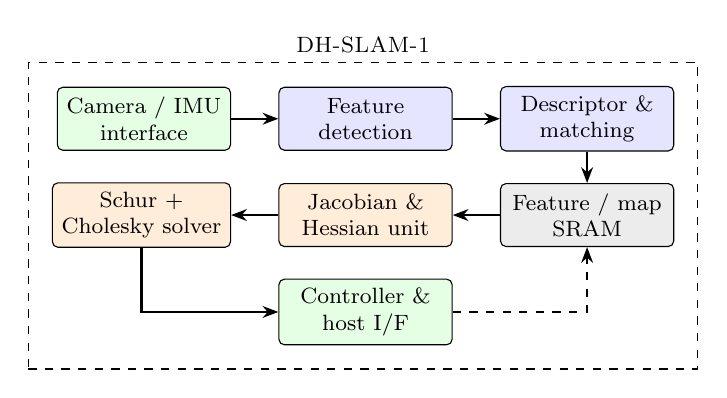
\begin{tikzpicture}[
    node distance = 4mm and 6mm,
    blk/.style  = {draw, rounded corners=2pt, minimum width=22mm,
                   minimum height=8mm, align=center, font=\footnotesize},
    fe/.style   = {blk, fill=blue!10},
    be/.style   = {blk, fill=orange!15},
    mem/.style  = {blk, fill=gray!15},
    io/.style   = {blk, fill=green!10},
    arr/.style  = {-{Stealth[length=2mm]}, thick},
  ]
  \node[io]  (cam)  {Camera / IMU\\interface};
  \node[fe, right=of cam]  (det)  {Feature\\detection};
  \node[fe, right=of det]  (trk)  {Descriptor \&\\matching};
  \node[mem, below=of trk] (fbuf) {Feature / map\\SRAM};
  \node[be, left=of fbuf]  (jac)  {Jacobian \&\\Hessian unit};
  \node[be, left=of jac]   (sol)  {Schur +\\Cholesky solver};
  \node[io, below=of jac]  (ctrl) {Controller \&\\host I/F};

  \draw[arr] (cam) -- (det);
  \draw[arr] (det) -- (trk);
  \draw[arr] (trk) -- (fbuf);
  \draw[arr] (fbuf) -- (jac);
  \draw[arr] (jac) -- (sol);
  \draw[arr] (sol) |- (ctrl);
  \draw[arr, dashed] (ctrl) -| (fbuf);

  \begin{scope}[on background layer]
    \node[draw, dashed, inner sep=3mm, fit=(det)(trk)(fbuf)(jac)(sol)(ctrl),
          label={[font=\footnotesize\itshape]above:\sysname}] {};
  \end{scope}
\end{tikzpicture}%
}

  \caption{Top-level architecture of \sysname.}
  \label{fig:arch}
\end{figure}

\subsection{Algorithm--Hardware Co-Design}
\label{sec:arch:codesign}
\TODO{Hardware-friendly modifications of the algorithm: fixed-point
formats (Q-format per signal), approximations, reduced descriptor length,
sliding-window size. Quantify their accuracy impact (refer to
\cref{sec:eval:accuracy}).}

\subsection{Front-End: Feature Extraction and Tracking}
\label{sec:arch:frontend}
\TODO{Streaming pipeline, line buffers, FAST/Harris detector, NMS,
descriptor/patch computation, matching engine, throughput (pixels/cycle).}

\subsection{Back-End: Optimization Engine}
\label{sec:arch:backend}
\TODO{Jacobian/Hessian construction unit, Schur complement, Cholesky solver,
marginalization; PE array organization; sparsity exploitation.}

\begin{algorithm}[t]
  \caption{Sliding-window Gauss--Newton (hardware schedule)}
  \label{alg:gn}
  \begin{algorithmic}[1]
    \Require Window states $\state$, measurements $\{\meas_{ij}\}$
    \For{$it = 1$ \textbf{to} $N_{\text{iter}}$}
      \State Compute residuals and Jacobians $\jac$ \Comment{Jacobian unit}
      \State Accumulate $\hess \gets \jac^\top\infomat\jac$, $\mathbf{b} \gets \jac^\top\infomat\mathbf{r}$
      \State Schur complement on landmark block \Comment{Schur unit}
      \State Solve reduced system by Cholesky \Comment{Solver}
      \State Back-substitute and update $\state \gets \state \boxplus \Delta\state$
    \EndFor
    \State Marginalize oldest keyframe
  \end{algorithmic}
\end{algorithm}

\subsection{Memory Hierarchy and Dataflow}
\label{sec:arch:memory}
\TODO{On-chip SRAM banks, sizes, bandwidth, data reuse, off-chip DRAM
traffic (if any), double buffering.}

\subsection{Control and Host Interface}
\TODO{Controller (FSM / RISC-V core), configuration registers, SPI/MIPI.}

% =============================================================================
\section{Implementation}
\label{sec:implementation}
% =============================================================================

\subsection{Design Flow}
\TODO{RTL language (SystemVerilog/Chisel/HLS), verification against
bit-accurate C++/Python model, synthesis and P\&R tools, PDK, standard-cell
library, SRAM compilers.}

\subsection{Chip Summary}
\Cref{tab:chip} summarizes the main characteristics of the fabricated chip,
and \cref{fig:die} shows the die micrograph.

\begin{table}[t]
  \centering
  \caption{Chip summary.}
  \label{tab:chip}
  % Сводка параметров чипа. \NUM — заглушка для чисел.
\small
\begin{tabular}{@{}ll@{}}
  \toprule
  Parameter            & Value \\
  \midrule
  Technology           & \NUM~nm CMOS \\
  Die area             & \NUM~\si{\milli\metre\squared} \\
  Core area            & \NUM~\si{\milli\metre\squared} \\
  On-chip SRAM         & \NUM~\si{\kilo\byte} \\
  Supply voltage       & \NUM--\NUM~\si{\volt} \\
  Clock frequency      & \NUM--\NUM~\si{\mega\hertz} \\
  Input resolution     & $640\times480$ \\
  Throughput           & \NUM\fps \\
  Power                & \NUM~\si{\milli\watt} \\
  Energy per frame     & \NUM\mJpf \\
  \bottomrule
\end{tabular}

\end{table}

\begin{figure}[t]
  \centering
  % \includegraphics[width=0.8\columnwidth]{die_photo.jpg}
  \fbox{\parbox[c][4cm][c]{0.8\columnwidth}{\centering
        \TODO{Die micrograph / layout with annotated blocks}}}
  \caption{Die micrograph of \sysname\ with annotated functional blocks.}
  \label{fig:die}
\end{figure}

\subsection{Area and Power Breakdown}
\TODO{Pie charts or stacked bars: area/power per block (front-end,
back-end, SRAM, control, I/O).}

\subsection{Test Setup}
\TODO{Measurement board, FPGA host, clock source, power measurement method,
sensor data playback.}

% =============================================================================
\section{Experimental Evaluation}
\label{sec:evaluation}
% =============================================================================

\subsection{Methodology}
\label{sec:eval:method}
\paragraph{Datasets.}
We evaluate on EuRoC MAV~\cite{burri2016euroc} and
TUM RGB-D~\cite{sturm2012tum} \TODO{(+ KITTI / own dataset?)}.

\paragraph{Metrics.}
Accuracy is measured by absolute trajectory error (ATE) and relative pose
error (RPE)~\cite{sturm2012tum}; hardware efficiency by throughput (FPS),
latency, power, energy per frame and area.

\paragraph{Baselines.}
\TODO{Software on ARM Cortex-A / x86, embedded GPU (Jetson), FPGA designs,
prior ASICs.}

\subsection{Accuracy}
\label{sec:eval:accuracy}
\TODO{ATE/RPE table: floating-point reference vs.\ fixed-point model vs.\
chip measurements, per sequence.}

\begin{table}[t]
  \centering
  \caption{ATE RMSE (\si{\metre}) on EuRoC sequences.}
  \label{tab:accuracy}
  % Точность (ATE RMSE, м). Колонки: эталон FP32, бит-точная модель, измерения на чипе.
\small
\begin{tabular}{@{}lccc@{}}
  \toprule
  Sequence & FP32 ref. & Fixed-point & \sysname \\
  \midrule
  MH\_01 & \NUM & \NUM & \NUM \\
  MH\_03 & \NUM & \NUM & \NUM \\
  MH\_05 & \NUM & \NUM & \NUM \\
  V1\_02 & \NUM & \NUM & \NUM \\
  V2\_02 & \NUM & \NUM & \NUM \\
  \midrule
  Mean   & \NUM & \NUM & \NUM \\
  \bottomrule
\end{tabular}

\end{table}

\subsection{Performance and Energy Efficiency}
\label{sec:eval:perf}
\TODO{Throughput and energy vs.\ baselines; voltage/frequency scaling
(shmoo plot); energy per frame breakdown.}

\subsection{Ablation Study}
\TODO{Contribution of each optimization (e.g., without streaming front-end,
without sparsity exploitation, different window sizes).}

\subsection{Comparison with State of the Art}
\label{sec:eval:sota}
\Cref{tab:sota} compares \sysname\ with previously published accelerators.

\begin{table*}[t]
  \centering
  \caption{Comparison with state-of-the-art SLAM/VIO accelerators.}
  \label{tab:sota}
  % Сравнение с SOTA (таблица на всю ширину страницы, table*).
\small
\begin{threeparttable}
\begin{tabular}{@{}lccccc@{}}
  \toprule
                       & Navion~\cite{suleiman2019navion} & \TODO{Work B} & \TODO{Work C} & \TODO{FPGA} & \textbf{\sysname} \\
  \midrule
  Technology (nm)      & 65   & \NUM & \NUM & --   & \NUM \\
  Algorithm            & VIO  & \NUM & \NUM & \NUM & \TODO{VI-SLAM} \\
  Loop closure         & No   & \NUM & \NUM & \NUM & \TODO{Yes/No} \\
  Area (mm$^2$)        & \NUM & \NUM & \NUM & --   & \NUM \\
  Frequency (MHz)      & \NUM & \NUM & \NUM & \NUM & \NUM \\
  Resolution           & \NUM & \NUM & \NUM & \NUM & $640\times480$ \\
  Frame rate (FPS)     & \NUM & \NUM & \NUM & \NUM & \NUM \\
  Power (mW)           & \NUM & \NUM & \NUM & \NUM & \NUM \\
  Energy/frame (mJ)    & \NUM & \NUM & \NUM & \NUM & \NUM \\
  Measured?            & Yes  & \NUM & \NUM & \NUM & Yes \\
  \bottomrule
\end{tabular}
\begin{tablenotes}\footnotesize
  \item \TODO{Notes: technology scaling assumptions, simulated vs.\ measured.}
\end{tablenotes}
\end{threeparttable}

\end{table*}

% =============================================================================
\section{Discussion}
\label{sec:discussion}
% =============================================================================

\paragraph{Limitations.}
\TODO{What is not supported (e.g., dense mapping, large-scale loop closure,
high resolution), robustness in challenging conditions, fixed sensor
configuration.}

\paragraph{Scalability.}
\TODO{How the architecture scales with resolution, window size, number of
landmarks, process node.}

\paragraph{Generality.}
\TODO{Applicability of the back-end engine to other factor-graph problems
(e.g., planning, calibration, sensor fusion).}

% =============================================================================
\section{Conclusion}
\label{sec:conclusion}
% =============================================================================
We presented \sysname, \TODO{one-sentence restatement of the system}.
\TODO{Main results with numbers: \NUM\fps, \NUM~\si{\milli\watt},
\NUM$\times$ energy-efficiency improvement, ATE \NUM~\si{\centi\metre}.}
\TODO{Future work: e.g., integrating loop closure, learned features,
next tape-out.}


\section*{Acknowledgments}
\TODO{Funding sources, grants, tape-out shuttle program, colleagues.}

\bibliographystyle{plainnat}
\bibliography{references}

\clearpage
\appendix
% =============================================================================
\section{Supplementary Material}
\label{sec:appendix}
% =============================================================================

\subsection{Fixed-Point Format Details}
\TODO{Table of Q-formats per signal and quantization error analysis.}

\subsection{Additional Results}
\TODO{Per-sequence trajectories, extra plots.}

\subsection{RTL Snippet}
\begin{lstlisting}[language=Verilog,caption={Example: pipelined MAC unit (placeholder).}]
module mac #(parameter W = 16) (
  input  logic                 clk, rst_n, en,
  input  logic signed [W-1:0]  a, b,
  output logic signed [2*W+7:0] acc
);
  always_ff @(posedge clk or negedge rst_n)
    if (!rst_n)  acc <= '0;
    else if (en) acc <= acc + a * b;
endmodule
\end{lstlisting}


\end{document}
